\chapter{Experimentos y resultados}
\doublespacing
\section{Experimentos}

Una vez entrenados, los modelos fueron evaluados utilizando un conjunto de datos de prueba para medir su rendimiento en términos de las métricas descritas en las ecuaciones \ref{eq:miou} - \ref{eq:dice_coefficient}. Esta evaluación permitió comprobar la efectividad de los modelos propuestos, asegurando que los resultados obtenidos fueran representativos de su capacidad para generalizar y segmentar adecuadamente en diferentes escenarios.

En las Figuras \ref{fig:Miou_vs_epochs}, \ref{fig:PA_vs_epochs} y \ref{fig:DICE_vs_epochs}, se muestran los resultados de las métricas MIoU (Mean Intersection over Union), PA (Pixel Accuracy) y Dice Coefficient (Dice) evaluadas para cada modelo CNN utilizando los datos de evaluación. 

\begin{figure}[h!]
	\centering
	\includegraphics[width=0.7\linewidth]{graficos/Miou_vs_epochs}
	\caption[Resultado del indicador MIou evaluado para cada modelo.]{Resultado del indicador MIou evaluado para cada modelo.
	}
	\label{fig:Miou_vs_epochs}
\end{figure}

\begin{figure}[h!]
	\centering
	\includegraphics[width=0.7\linewidth]{graficos/PA_vs_epochs}
	\caption[Resultado del indicador PA evaluado para cada modelo.]{Resultado del indicador PA evaluado para cada modelo.
	}
	\label{fig:PA_vs_epochs}
\end{figure}

\begin{figure}[h!]
	\centering
	\includegraphics[width=0.7\linewidth]{graficos/DICE_vs_epochs}
	\caption[Resultado del indicador Dice evaluado para cada modelo.]{Resultado del indicador Dice evaluado para cada modelo.
	}
	\label{fig:DICE_vs_epochs}
\end{figure}

\begin{figure}[h!]
	\centering
	\includegraphics[width=0.7\linewidth]{graficos/Loss_vs_epochs}
	\caption[Resultado de convergencia de la función de pérdida (Loss) evaluado para cada modelo.]{Resultado de convergencia de la función de pérdida evaluado para cada modelo.
	}
	\label{fig:Loss_vs_epochs}
\end{figure}

Los modelos fueron evaluados utilizando un conjunto de datos de prueba compuesto por 360 imágenes, aplicando métricas como mIoU, Dice Coefficient, y PA para medir la precisión. Los resultados cuantitativos se presentan en la tabla \ref{tabla3}.
%,donde se observa que DeepLabV3Plus obtuvo el rendimiento más bajo en la segmentación según las métricas. Por otro lado, DeepResUnet mostró una mejora considerable en comparación con DeepLabV3Plus al evaluar las mismas imágenes y métricas. Sin embargo, U-Net fue el modelo que alcanzó los mejores resultados en la segmentación de cuerpos glaciares.

%Basado en la integración de las bandas 2, 3, 4, 5, 6 y 7 para Landsat 8 y las bandas 1,2,3,4,5,7 para landsat 5 Collection 2 Level-1, U-Net demostró ser el modelo con el mejor rendimiento, mostrando una gran precisión en la clasificación y segmentación de los límites de una amplia variedad de glaciares.

%No obstante, ResUnet tambien presenta un comportamiento muy similar a U-Net. Sin embargo; este modelo presenta el mayor número de parámetros de entrenamiento en comparación con U-Net y DeepLabV3+, lo que se atribuye al mecanismo residual, que, aunque mejora el rendimiento, incrementa el costo computacional.

\begin{table}[h!]
	\centering
	\begin{tabular}{|c|c|c|c|c|}
		\hline
		\textbf{Modelo} & \textbf{Loss} &\textbf{Miou} & \textbf{PA} & \textbf{Dice Coefficient}\\
		\hline
		U-Net  & 0.0100 & 0.9810 & 0.9979 & 0.9904  \\
		ResUnet   & 0.0113 & 0.9782 & 0.9963 & 0.9882 \\
		DeepLabV3+ & 0.0704 & 0.8541 & 0.9824  & 0.9199 \\
		
		\hline
	\end{tabular}
	\caption{Párametros de entrenamiento}
	\label{tabla3}
\end{table}

Finalmente, U-Net demuestra un menor valor de pérdida y mayores puntajes en las métricas MIoU, PA y Dice Coefficient, consolidándose como el modelo más adecuado para tareas de segmentación semántica de cuerpos glaciares en el Perú.

La Figura \ref{fig:comparative_predictions} se muestra los resultados de segmentación obtenidos por los modelos propuestos. %DeepLabV3Plus no logró segmentar los cuerpos glaciares con suficiente detalle, aunque presentó un comportamiento aceptable en general. Por su parte, el modelo DeepResUnet logró segmentar los límites de los cuerpos glaciares de manera más completa, mostrando un rendimiento superior en comparación con DeepLabV3+. Sin embargo, el mejor desempeño fue alcanzado por U-Net, que ofreció una segmentación más precisa y exacta de los límites glaciares, reflejando su capacidad para capturar detalles con mayor fidelidad.


\begin{figure}[h!]
	\centering
	\includegraphics[width=\linewidth]{graficos/comparative_predictions}
	\caption[Análisis cualitativo y cuantitativo de los modelos eveluados.]{Cualitativamente, tanto U-Net como ResUnet muestran una gran similitud con las máscaras de referencia, logrando segmentar con precisión los bordes de los cuerpos glaciares. En contraste, aunque DeepLabV3Plus logra una segmentación aceptable, no alcanza el mismo nivel de precisión en la delimitación de los bordes.
		Cuantitativamente, U-Net muestra un rendimiento sobresaliente, mientras que DeepResUnet ofrece un rendimiento competitivo. En comparación, DeepLabV3Plus no alcanza un nivel competitivo frente a los otros modelos.
		
	}
	\label{fig:comparative_predictions}
\end{figure}




El enfoque utilizado para el análisis temporal, con el fin de reducir la influencia de la nieve efímera, consistió en analizar múltiples escenas durante la estación seca y seleccionar aquellas que mejor representaran la extensión del glaciar. Para ello, se eligieron únicamente escenas sin nieve efímera visible en el paisaje circundante al glaciar, aplicando una técnica de preselección común.

\subsection{Evolución del glaciar Quelccaya}

Posteriormente, se creó un conjunto de datos que incluye únicamente las imágenes del glaciar Quelccaya, seleccionando las más representativas de los años de interés. Este dataset fue preprocesado y utilizado como entrada para la red neuronal U-Net, con el objetivo de generar imágenes predichas que luego se emplearían para calcular el área del glaciar en cada año.

Dado que la red neuronal acepta entradas de tamaño 256x256, fue necesario reconstruir las imágenes predichas a un tamaño de 512x512, adecuado para contener la totalidad del glaciar Quelccaya. Una vez reconstruida, la imagen resultante es completamente binaria, con un tamaño de 512x512, donde los píxeles blancos segmentados representan los cuerpos glaciares y los píxeles negros cualquier otra superficie.

Cada imagen binaria se procesa sumando los píxeles blancos, considerando que cada píxel tiene una resolución de 30 metros. De esta manera, se calcula el área del glaciar correspondiente a cada año. Este procedimiento se repite para los demás años de interés.


\begin{figure}[h!]
	\centering
	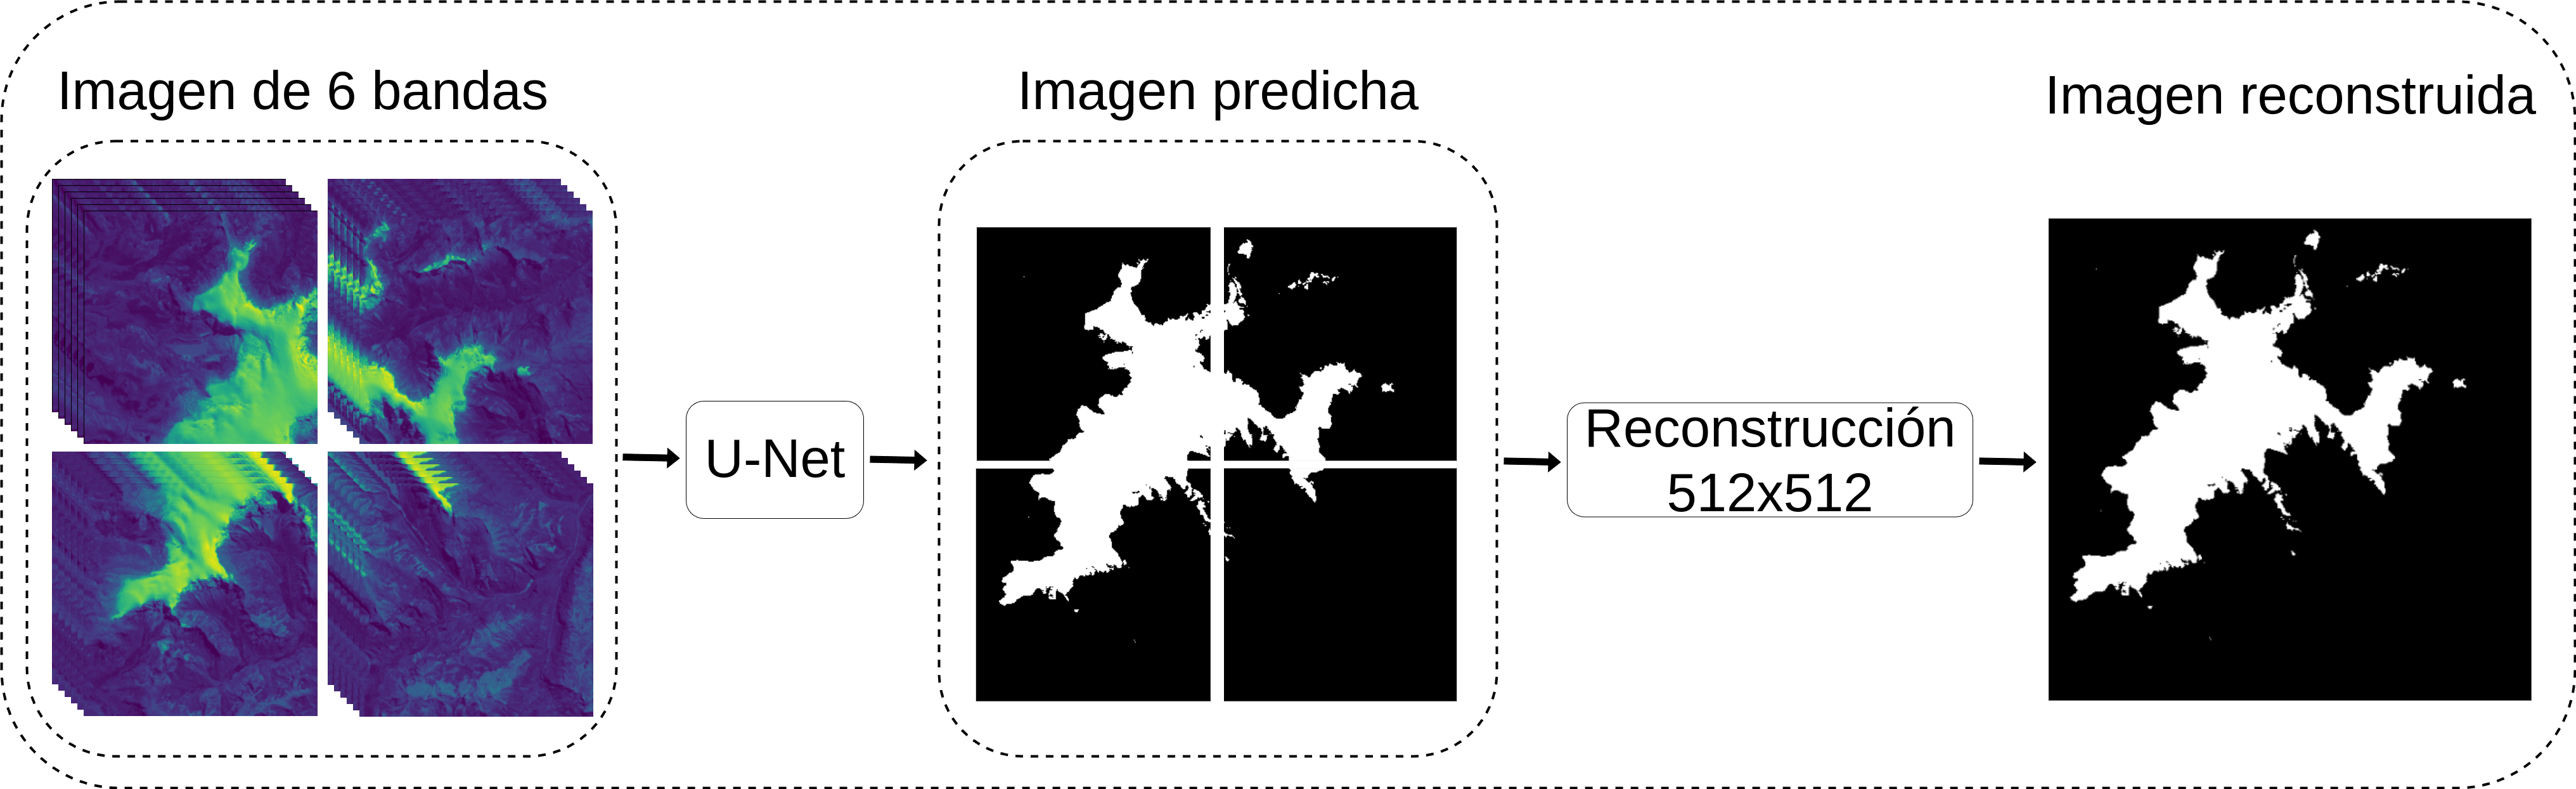
\includegraphics[width=\linewidth]{graficos/reconstruir_imagen}
	\caption[Proceso de predicción y reconstrucción para calcular el área segmentada.]{Proceso de predicción y reconstrucción para calcular el área segmentada.
		
	}
	\label{fig:reconstruir_imagen}
\end{figure}


%La Figura \ref{fig:imagen_temporal} se muestran imagenes binarias los cuales nos indican como el glaciar Quelccaya disminuyo en área, se puede visualizar que algunos cuerpos glaciares disminuyeron drasticamente durante el tiempo hasta llegar a desaparecer, tal como se muestra en la Figura \ref{fig:comparacion}, en la imagen del año 1991 en el recuadro rojo aun se puede observar la existencia de cuerpo glaciares, en el año 2010 estos cuerpos glaciares aun mantenian presencia escasa y en la actualidad para el año 2024 se puede observar que estos cuerpos glaciares desaparecieron completamente. 


La Figura \ref{fig:imagen_temporal} muestra imágenes binarias que evidencian la reducción en el área del glaciar Quelccaya a lo largo del tiempo. En particular, se observa que algunos cuerpos glaciares disminuyeron drásticamente hasta desaparecer por completo, como se ilustra en la Figura \ref{fig:comparacion} donde se observa que en la imagen de 1991, el recuadro rojo destaca la presencia de estos cuerpos glaciares; en 2010, aunque aún son visibles, su extensión es muy reducida. Para el año 2024, estos cuerpos glaciares han desaparecido completamente.


\begin{figure}[h!]
	\centering
	\includegraphics[width=\linewidth]{graficos/imagen_temporal}
	\caption[Retroceso superficial del glaciar Quelccaya.]{Retroceso superficial del glaciar Quelccaya vizualizada mediante imagenes binarias segmentadas utilizando el modelo U-Net.
		
	}
	\label{fig:imagen_temporal}
\end{figure}

\begin{figure}[h!]
	\centering
	\includegraphics[width=\linewidth]{graficos/comparacion}
	\caption[Cuerpos glaciares extintos.]{El recuadro rojo encierra cuerpos glaciares que se extingieron gradulamente hasta llegar a desaparecer completamente.
		
	}
	\label{fig:comparacion}
\end{figure}



En la figura \ref{fig:predicciones_temporales}, se visualizan los cambios en la superficie del glaciar Quelccaya para los años 1991, 2006 y 2024, con el propósito de proporcionar una mejor representación del retroceso glaciar. En esta figura se muestran los bordes correspondientes a cada año: el borde azul indica la extensión del glaciar en 1991, el borde rojo en 2006 y el borde rosado en 2024. 

Es importante mencionar que para delinear los bordes de los glaciares en distintos años se empleó el algoritmo de Canny, ampliamente utilizado para detectar todos los contornos presentes en una imagen. En este caso, el algoritmo identifica los bordes de los glaciares a partir de una imagen binaria, permitiendo observar los cambios en su extensión a lo largo del tiempo.

\begin{figure}[h!]
	\centering
	\includegraphics[width=\linewidth]{graficos/predicciones_temporales}
	\caption[Contornos glaciares más antiguos y mas recientes del glaciar Quelccaya.]{Contornos glaciares más antiguos y mas recientes del glaciar Quelccaya.
		
	}
	\label{fig:predicciones_temporales}
\end{figure}






%Se ha realizado una gráfica de la serie temporal tal como se muestra en la figura, para cuantificar el retroceso glaciar. Los resultados indican que la superficie del glaciar Quelccaya ha disminuido notablemente en un 30.15\% durante el periodo 1991-2024, pasando de 50.81 km² en 1991 a 35.49 km² en 2024. Esto representa una tasa de disminución de 0.424 ± 0.136 km²/año, con todas las incertidumbres expresadas como intervalos de confianza del 95 \%.En el análisis se excluyeron algunos años, ya que se comprobó que no representaban con precisión la extensión de la capa de hielo. Estos años mostraban áreas anómalas, probablemente debido a la presencia de nieve efímera, una fuente potencialmente significativa de inexactitud al analizar escenas con esta cobertura temporal.

%\subsection{Comparación con trabajos previos}

%Los antecedentes sobre estimulación del area del glacear Quelccaya son muy escasas la mayoria de los estudios limitan su analisis a estudiar regiones mucho mas amplia. Ademas los limites glaciares analizados no son fijos, puesto que en la mayoria de los casos los autores suelen elegir manualmente las imagens satelitales que podrian no contener nieve temporal para evitar resultados inadecuados, para comparar los resultados obtenidos de esta investigación se concidera los estudios realizados por \parencite{malone2022evolution}, \parencite{taylor2022multi} y \parencite{hanshaw2014glacial}, donde \parencite{malone2022evolution} y \parencite{taylor2022multi} son estudios recientes que incluyen es estudio temporal del glaciar Quelccaya. Los resultados de la estimacion de áreas glacear de esta investigación para el glaciar Quelccaya llegan a tener valores muy cercanos a los antecedentes y en alghunos años el valor de área glaciar incluso fue muy proximo a los antecedentes, tal es el caso de los años 1991, 1992, 1995, 1999, 2006, 2009, 2015, 2019, 2020, En la figura se puede observar que algunos valores de área glaciar de este estudio son muy cercanos y aun logran superponerse, de igual forma hay algunos valores que son ligeramente alejados, pero en general la mayoria de los datos llegan a estar muy proximos a los antecedentes. ademas los resultados en general son mucho mas comparables y similares a los resultados de \parencite{malone2022evolution} sn embargo, suele existir discrepancias en algunos valores que probablemente se deba a la forma de trazado de limites de los glaciares, el estudio actual informa datos cuenta con datos con una resolución de 30 metros. Para Los resultados del el año 2020, año en que finaliso el analsis para \parencite{taylor2022multi} y \parencite{malone2022evolution},  se obtubo un area glaciar de  41.58 km² para \parencite{taylor2022multi}, de 39.03 km² para \parencite{malone2022evolution}  y para este estudio es de el area obtenida fue de 38.99 km², la tasa de retroceso glaciar para \parencite{malone2022evolution} fue de 0.43 km²/año, mientras que para esta investigación la tasa de retroceso glaciar es de 0.3935 km²/año, sin embargo este estudio extendio el analisis temporal hasta 2024 llegando a tener un area de 35.49 km².

\section{Resultados}

Los resultados indican que la superficie del glaciar Quelccaya ha disminuido notablemente en un 30.15\% durante el periodo 1991-2024, pasando de 50.81 km² en 1991 a 35.49 km² en 2024. Esto representa una tasa de disminución de 0.38.99 km²/año, con todas las incertidumbres expresadas como intervalos de confianza del 93 \%. En área superficial del año actual 2024 es una versión más pequeña y más restringida a su versión de 1991. 

En el análisis se excluyeron algunos años, ya que se comprobó que no representaban con precisión la extensión de la capa de hielo. Estos años mostraban áreas anómalas, probablemente debido a la presencia de nieve efímera, una fuente potencialmente significativa de inexactitud al analizar escenas con esta cobertura temporal.

\begin{table}[h!]
	\centering
	\begin{tabular}{|c|c|}
		\hline
		\textbf{Año} & \textbf{Área glaciar (km²)} \\
		\hline
		1991 & 50.8131  \\
		1992 & 49.4514  \\
		1995 & 48.7134  \\
		1996 & 47.2077  \\
		1997 & 48.2877  \\
		1999 & 46.2609  \\
		2003 & 45.4023  \\
		2005 & 42.7689  \\
		2006 & 44.1945  \\
		2007 & 42.3459  \\
		2008 & 42.0192  \\
		2009 & 41.4171  \\
		2010 & 40.0995  \\
		2014 & 43.3746  \\
		2015 & 41.5998  \\
		2016 & 39.2517  \\
		2017 & 39.0825  \\
		2019 & 38.4210 \\
		2020 & 38.9988  \\
		2021 & 39.6297  \\
		2022 & 37.9539  \\
		2023 & 37.2051  \\
		2024 & 35.4951  \\
	
		
		
		\hline
	\end{tabular}
	\caption{Resultado cuantitativo de la estimación de superficie glaciar a travez del tiempo}
	\label{tabla5.1}
\end{table}

\begin{figure}[h!]
	\centering
	\includegraphics[width=\linewidth]{graficos/grafica_regresion1}
	\caption[Análisis temporal del glaciar Quelccaya.]{Análisis temporal del glaciar Quelccaya.
		
	}
	\label{fig:grafica_regresion}
\end{figure}

\singlespacing